% \documentclass{article}
% \usepackage[utf8]{inputenc}

% \title{AProf Hw1}
% \author{André Lopes Rodrigues}
% \author{Duarte Calado Almeida}
% \date{December 2022}

% \begin{document}

% \maketitle

% \section{Introduction}

% \end{document}

\documentclass{exam}

\usepackage{titling}
\usepackage{amsmath}
\usepackage{amsfonts}
\usepackage{mathtools}
\usepackage{float}
\usepackage{tikz}
\usepackage{graphicx}
\usepackage{subfig}
\usepackage{inconsolata}
\usepackage{tikz}
\usepackage{physics}
\usepackage{amsthm}
\usepackage[font={small}]{caption}
\usepackage{courier}

\graphicspath{ {./pictures} }

\setlength{\droptitle}{-5em}   

%\renewcommand{\questionlabel}{\textbf{~\thequestion)}}
%\renewcommand{\subpartlabel}{\thesubpart)}
%\DeclarePairedDelimiterX{\norm}[1]{\lVert}{\rVert}{#1}

\newcommand*{\horzbar}{\rule[.5ex]{2.5ex}{0.5pt}}

\newenvironment{shiftedflalign*}{%
    \start@align\tw@\st@rredtrue\m@ne
    \hskip\parindent
}{%
    \endalign
}

\newcommand{\brows}[1]{%
  \begin{bmatrix}
  \begin{array}{@{\protect\rotvert\;}c@{\;\protect\rotvert}}
  #1
  \end{array}
  \end{bmatrix}
}

\newcommand{\rotvert}{\rotatebox[origin=c]{90}{$\vert$}}
\newcommand{\rowsvdots}{\multicolumn{1}{@{}c@{}}{\vdots}}

\newtheorem{lemma}{Lemma}

\title{%
  Homework 2\\
  \vspace{0.5em}
  \large Deep Learning }
\author{
  Duarte Calado de Almeida\\
  95565
  \and
  André Lopes Rodrigues\\
  96576
}
\date{}

\cfoot{\thepage}

\begin{document}
    \maketitle
    
    \begin{tikzpicture}[overlay, remember picture]
        \node[xshift=3.5cm,yshift=-2cm] at (current page.north west) {
\includegraphics[scale = 0.35]{logo_ist.jpg}};
    \end{tikzpicture}

    \vspace{-3em}

    \noindent\makebox[\linewidth]{\rule{18cm}{0.4pt}}

        The contribution of each member was as follows:\\
        % André Rodrigues did Questions 1.1 and 2, 
        % while Duarte Almeida did Questions 1.2 and 3. The elaboration of this report was made in colaboration by both students.
    % \vspace{-0.5cm}
    \noindent\makebox[\linewidth]{\rule[1ex]{18cm}{0.4pt}}
    

    \section*{Question 1}
    \begin{questions}
        \question
        \begin{parts}
            \part %1.1(a)
                z has dimensions (H-M+1)*(W-N+1)
            
            \part %1.1(b)
                Matriz toda fudida    

            \part %1.1(c)
                
                
        \end{parts}
        %\newpage
        \question 
            procurar nos slides por single head self attention layer        

    \end{questions}

    \section*{Question 2}

    \begin{questions}
        \question %2.1
       
        \question %2.2

        \question %2.3

        \question
        The convolutional network was implemented and tested for 20 epochs, using Adam tuning with the following learning rate values.
        
        \begin{table}[h!]
            \centering
            \begin{tabular}{c|ccccc}
                &                                     & Learning Rate                      &                 &  &  \\ \cline{2-4}
                & \multicolumn{1}{c|}{0.00001}          & \multicolumn{1}{c|}{0.0005}          & 0.01             &  &  \\ \cline{1-4}
                Validation Accuracy & \multicolumn{1}{c|}{0.9559} & \multicolumn{1}{c|}{0.9843} & 0.7516 &  & 
            \end{tabular}
        \end{table}
    
        The best observed configuration was the one with a learning rate of 0.0005.
        The plots of the training loss and validation accuracy over the number of epochs are shown below.

        \begin{figure}[H]
            \centering
            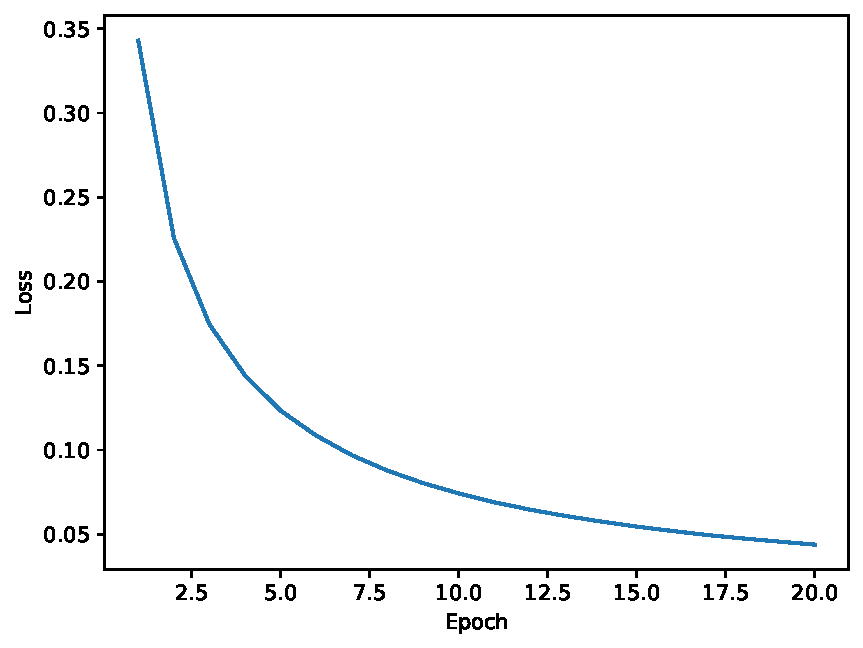
\includegraphics[scale=0.6]{CNN-training-loss-0.0005-0.3-0-adam.pdf}
            \caption{Training Loss over no. of epochs for $\eta = 0.0005$}
            \label{}
        \end{figure}

        \begin{figure}[H]
            \centering
            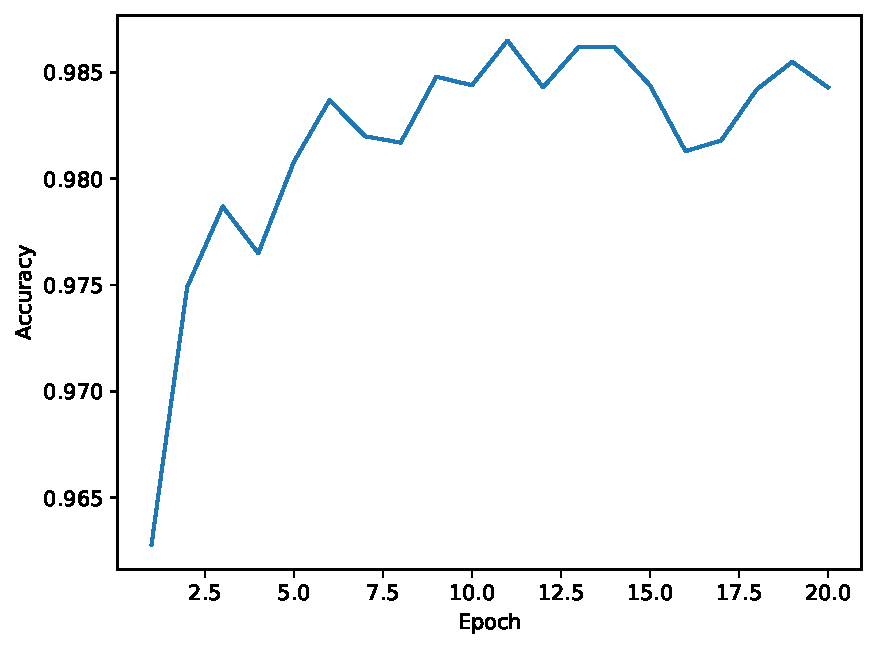
\includegraphics[scale=0.6]{CNN-validation-accuracy-0.0005-0.3-0-adam.pdf}
            \caption{Validation Accuracy over no. of epochs for $\eta = 0.0005$}
            \label{}
        \end{figure}

        \question
        The activation map 

        \begin{figure}[H]
            \centering
            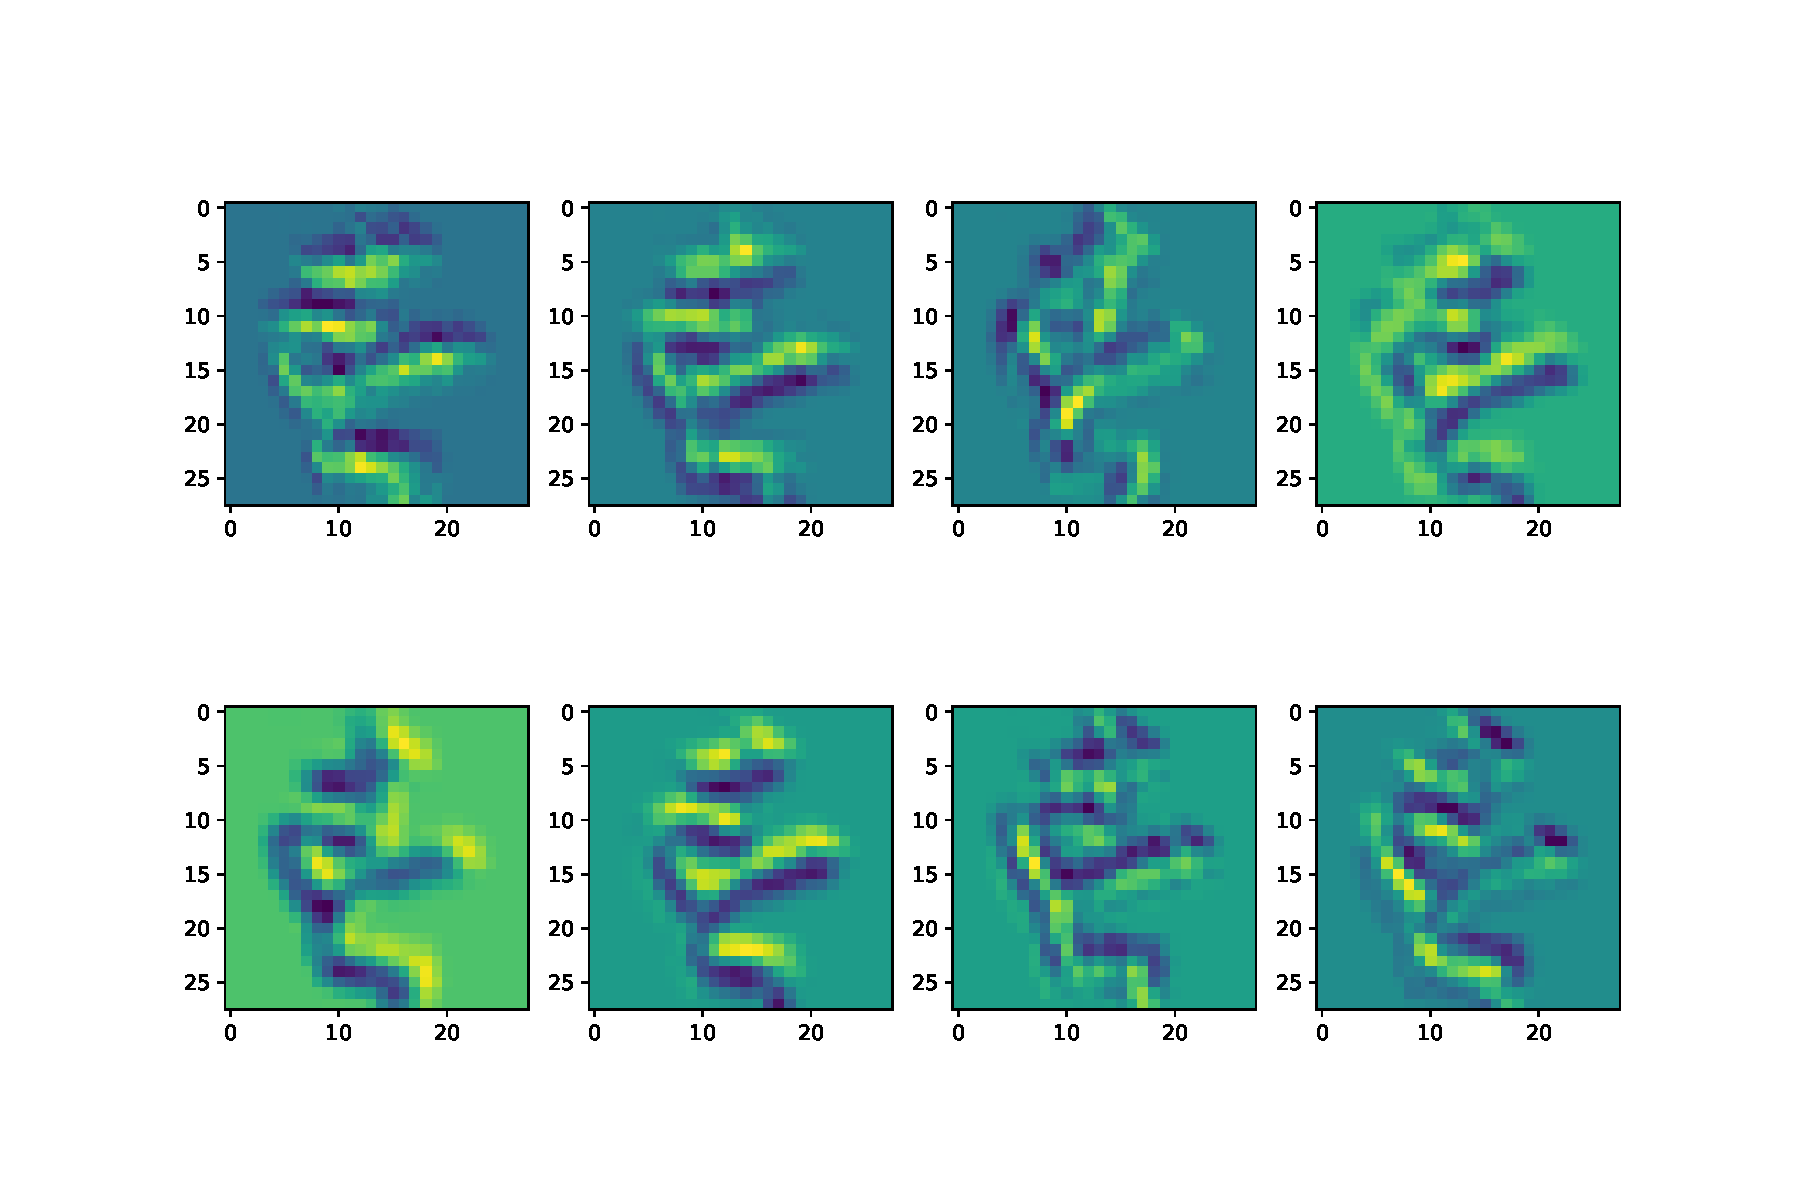
\includegraphics[scale=0.4]{activation_maps.pdf}
            \caption{Activation Maps of the first convolutional layer}
            \label{fig:activation}
        \end{figure}

        \begin{figure}[H]
            \centering
            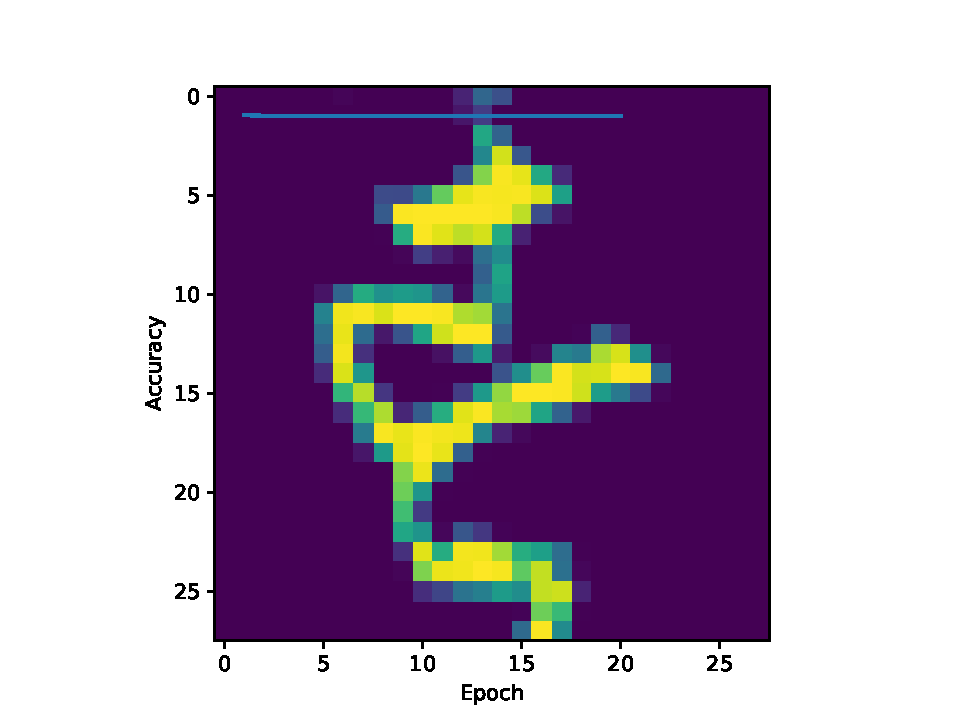
\includegraphics[scale=0.4]{original_image.pdf}
            \caption{Original Training Image}
            \label{fig:orig}
        \end{figure}

    \end{questions}

    \newpage

    \section*{Question 3}
    \begin{questions}
        \question
        \begin{parts}
            \part %3.1(a)

            \part %3.1(b)

            \part %3.1(c)


        \end{parts}
    \end{questions}
\end{document}